% ============================================================================
\section{Electric-Machine Requirements and Integrated Implementation}
\label{sec:machine_requirements}
% ============================================================================

% ---------------------------------------------------------------------------
\subsection{Winding Architecture and Electromagnetic Coupling}
% ---------------------------------------------------------------------------

Although the winding groups are electrically separated at their
terminals, they share the same magnetic circuit, rotor, air gap, and
shaft. 
Their electromagnetic coupling depends on winding distribution,
slot/pole combination, spatial displacement, and machine geometry
\cite{Che2014SeriesConnected,Bringezu2020SPB,
Verkroost2024PowerDistribution,Zhang2014SPBMachine}. 
Therefore, an SPB-compatible machine
cannot generally be obtained simply by dividing a conventional
three-phase winding into multiple groups without considering the
resulting coupling and harmonic behavior.

The three-phase groups may be aligned, 
spatially shifted, or implemented as physically segmented stator
modules. 
Spatial displacement affects mutual coupling, torque-ripple
components, and the additional current subspaces available to the
controller, among other effects
\cite{Zhang2025MultiphaseReview,Das2025SixPhaseWinding,
Wang2025DTPHarmonics}. 
These additional subspaces can introduce non-torque-producing currents,
 but they can also be exploited for
harmonic suppression, differential power sharing, and fault-tolerant
operation
\cite{Tang2025SixPhaseFault,Verkroost2024PowerDistribution}. 
Split winding architectures show a similar tradeoff: they can reduce ripple
and provide additional current/voltage degrees of freedom, but they do
so by increasing winding terminals and coupling complexity
\cite{Han2014SplitWindingModular}. These three winding-group
arrangements are compared schematically in
Fig.~\ref{fig:winding_options}.

\begin{figure*}[!t]
\centering
\resizebox{\textwidth}{!}{%
\begin{circuitikz}[font=\scriptsize,>=latex,x=1mm,y=1mm]
\ctikzset{bipoles/length=4mm}

% =====================================================================
% Panel (a): Aligned -- every slot hosts both groups, inner/outer layer.
% Long coil legs reaching close to the bore boundary and a shaft-only
% center marker (not a large rotor disk) so the content, not empty
% space, dominates the circle -- matching the reference proportions.
% =====================================================================
\begin{scope}[shift={(0,0)}]
\draw[fill=black!25] (0,0) circle (2.2);
\draw[black!40,thin] (0,0) circle (52);
\foreach \a in {90,210,330}{
\draw[black!20,thin] (\a:3) -- (\a:50.5);
\begin{scope}[shift={(\a:22)}]
\foreach \la/\lb in {90/A,210/B,330/C}{
  \draw[blue!55!black,ultra thick] (\la:1.2) to[cute inductor] (\la:9);
  \node[font=\small,blue!55!black] at (\la:11) {$\lb$1};
}
\node[circle,fill=blue!55!black,inner sep=0.8pt] at (0,0) {};
\end{scope}
\begin{scope}[shift={(\a:38)}]
\foreach \la/\lb in {90/A,210/B,330/C}{
  \draw[orange!70!black,ultra thick] (\la:1.2) to[cute inductor] (\la:9);
  \node[font=\small,orange!70!black] at (\la:11) {$\lb$2};
}
\node[circle,fill=orange!70!black,inner sep=0.8pt] at (0,0) {};
\end{scope}
}
\node[align=center] at (0,-60) {(a) Aligned};
\end{scope}

% =====================================================================
% Panel (b): Shifted -- both groups at the same radius, offset by
% Delta-theta so the six coil clusters interleave with long legs
% reaching close to the boundary
% =====================================================================
\begin{scope}[shift={(102,0)}]
\draw[fill=black!25] (0,0) circle (2.2);
\draw[black!40,thin] (0,0) circle (39);
\foreach \a in {90,210,330}{
\begin{scope}[shift={(\a:26)}]
\foreach \la/\lb in {90/A,210/B,330/C}{
  \draw[blue!55!black,ultra thick] (\la:1.2) to[cute inductor] (\la:9);
  \node[font=\small,blue!55!black] at (\la:11) {$\lb$1};
}
\node[circle,fill=blue!55!black,inner sep=0.8pt] at (0,0) {};
\end{scope}
\pgfmathsetmacro{\ashift}{\a+60}
\begin{scope}[shift={(\ashift:26)}]
\foreach \la/\lb in {90/A,210/B,330/C}{
  \draw[orange!70!black,ultra thick] (\la:1.2) to[cute inductor] (\la:9);
  \node[font=\small,orange!70!black] at (\la:11) {$\lb$2};
}
\node[circle,fill=orange!70!black,inner sep=0.8pt] at (0,0) {};
\end{scope}
}
\draw[->,thin,black!60] (120:36) arc[start angle=120,end angle=150,radius=36];
\node[font=\small] at (135:39) {$\Delta\theta$};
\node[align=center] at (0,-47) {(b) Shifted};
\end{scope}

% =====================================================================
% Panel (c): Segmented -- one shared bore, split into four physically
% separate modules (dashed radial boundaries) alternating group 1 and
% group 2, with the same long-leg coil size as (a)/(b)
% =====================================================================
\begin{scope}[shift={(204,0)}]
\draw[fill=black!25] (0,0) circle (2.2);
\draw[black!40,thin] (0,0) circle (39);
\foreach \b in {45,135,225,315}{
  \draw[black!40,thin,dashed] (\b:3) -- (\b:37.5);
}
\begin{scope}[shift={(0:26)}]
\foreach \la/\lb in {90/A1,210/B1,330/C1}{
  \draw[blue!55!black,ultra thick] (\la:1.2) to[cute inductor] (\la:9);
  \node[font=\small,blue!55!black] at (\la:11) {$\lb$};
}
\node[circle,fill=blue!55!black,inner sep=0.8pt] at (0,0) {};
\end{scope}
\begin{scope}[shift={(180:26)}]
\foreach \la/\lb in {90/A1,210/B1,330/C1}{
  \draw[blue!55!black,ultra thick] (\la:1.2) to[cute inductor] (\la:9);
  \node[font=\small,blue!55!black] at (\la:11) {$\lb$};
}
\node[circle,fill=blue!55!black,inner sep=0.8pt] at (0,0) {};
\end{scope}
\begin{scope}[shift={(90:26)}]
\foreach \la/\lb in {90/A2,210/B2,330/C2}{
  \draw[orange!70!black,ultra thick] (\la:1.2) to[cute inductor] (\la:9);
  \node[font=\small,orange!70!black] at (\la:11) {$\lb$};
}
\node[circle,fill=orange!70!black,inner sep=0.8pt] at (0,0) {};
\end{scope}
\begin{scope}[shift={(270:26)}]
\foreach \la/\lb in {90/A2,210/B2,330/C2}{
  \draw[orange!70!black,ultra thick] (\la:1.2) to[cute inductor] (\la:9);
  \node[font=\small,orange!70!black] at (\la:11) {$\lb$};
}
\node[circle,fill=orange!70!black,inner sep=0.8pt] at (0,0) {};
\end{scope}
\node[align=center] at (0,-47) {(c) Segmented};
\end{scope}

% ---- Legend ----
\node[circle,fill=blue!55!black,inner sep=1.4pt] at (72,-70) {};
\node[right,font=\small] at (73.8,-70) {Winding group 1};
\node[circle,fill=orange!70!black,inner sep=1.4pt] at (127,-70) {};
\node[right,font=\small] at (128.8,-70) {Winding group 2};
\node[fill=black!25,minimum size=2mm,inner sep=0] at (10,-70) {};
\node[right,font=\small] at (11.8,-70) {Shaft};
\end{circuitikz}}
\caption{Schematic comparison of the winding-group spatial arrangements
: (a)~aligned  groups (b)~spatially shifted groups and (c)~physically
segmented stator modules.}
\label{fig:winding_options}
\end{figure*}

For the $k$th PMSM winding group,

\begin{equation}
\begin{aligned}
v_{d,k}&=R_{s,k}i_{d,k}-\omega_{\mathrm e}L_{q,k}i_{q,k},\\
v_{q,k}&=R_{s,k}i_{q,k}
+\omega_{\mathrm e}\left(L_{d,k}i_{d,k}+\psi_{f,k}\right),
\end{aligned}
\label{eq:spb_machine_dq}
\end{equation}

and the required voltage must satisfy

\begin{equation}
\sqrt{v_{d,k}^{2}+v_{q,k}^{2}}
\leq
k_{\mathrm{mod}}V_{\mathrm{dc},k}
\approx
k_{\mathrm{mod}}\frac{V_{\mathrm{dc}}}{N}.
\label{eq:spb_machine_voltage_limit}
\end{equation}

This falling per-cell voltage budget ties winding turns, inductance,
and field-weakening capability directly to $N$ -- a coupling
demonstrated in optimized multiphase SPB-PMSM systems
\cite{Bringezu2020SPB}. Recent multiphase traction-machine studies
similarly emphasize coordinated design of winding voltage, harmonic
subspaces, and modulation
\cite{Chen2026HighModulationDTP,Feng2026TractionMachine}.

% ---------------------------------------------------------------------------
\subsection{From Multiphase Machine to Integrated Modular Drive}
% ---------------------------------------------------------------------------

Physical integration can convert the added electrical complexity of
many winding groups into a packaging advantage. With a remote
inverter, additional winding groups increase phase-cable and connector
count; positioning each converter bridge close to its corresponding
winding group instead reduces external cabling, shortens
high-frequency interconnections, distributes heat sources, and aligns
converter modules with stator segments.

This design philosophy predates SPB and has been extensively studied
in integrated and modular motor drives
\cite{Shakweh2002PlugPlayIMD,Wheeler2005Integrated30kW,
Pickering2006ThermalIMD,Brown2007IMMD,Wolmarans2008IntegratedFT,
Hennen2012DistributedIMMD,Choi2011IMMD,Wang2013GaNIMMD,
Wang2015GaNIMMD,Wang2025GaNIMMD,Ugur2018GaNIMMD,
Ugur2019MultiphysicsIMMD,Mohamed2021Electrothermal,
Mohamed2021EnhancedIMD,Mohamed2022IntegratedDCLink,Wang2025MWIMMD,
Chen2026WBGIMD,Deng2026IMDReview}, summarized in
Table~\ref{tab:immd_relevance}. The overall trend runs from early
cable-reduction and compact-packaging concepts through jointly
designed fault-tolerant converter/winding/thermal architectures and
series-connected GaN IMMDs to recent WBG-based axial-flux IMMDs
demonstrating stator-mounted converter modules and scalability to
MW-class and EV-traction implementations.

% ---------------------------------------------------------------------------
\subsection{Physical Integration Options}
\label{subsec:physical_integration}
% ---------------------------------------------------------------------------

The electrically separated winding groups required by SPB do not
impose a unique converter placement on a radial-flux machine. Chowdhury
\textit{et al.} \cite{Chowdhury2019Integration}, consistent with the
broader integrated-motor-drive survey of Abebe \textit{et al.}
\cite{Abebe2016IMDReview}, classify motor/inverter physical integration
into four categories: whether the converter mounts radially or
axially, and whether it interfaces with a separate housing/end-cap
structure or directly with the stator core. This taxonomy frames how
SPB converter cells can be placed around a radial-flux machine, as
illustrated in Fig.~\ref{fig:machine_integration}. The axial-flux
stator-mounted and polygon-housing alternative is covered by the
Mohamed \textit{et al.} developments
\cite{Mohamed2021Electrothermal,Mohamed2021EnhancedIMD,
Mohamed2022IntegratedDCLink} in Table~\ref{tab:immd_relevance}.


%\cite{Abebe2015FEAThermal}.

\begin{figure*}[!t]
\centering
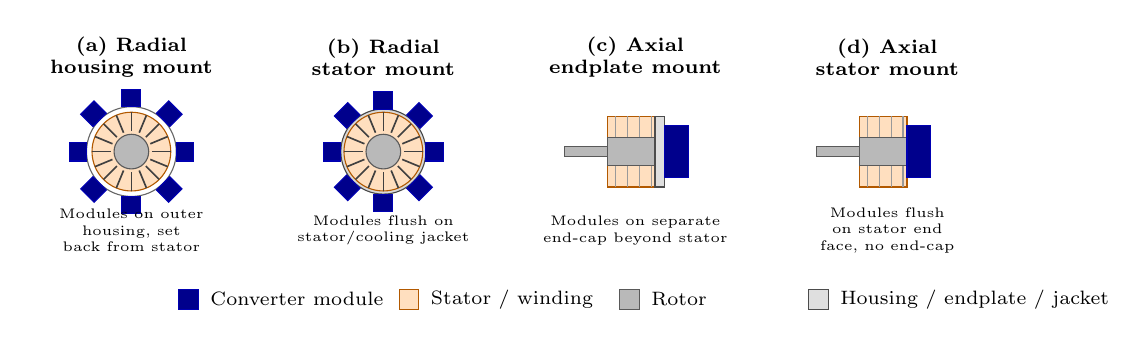
\begin{tikzpicture}[font=\scriptsize,>=latex,x=1mm,y=1mm]
% ================= Panel (a): Radial housing mount (radial cross-section) =================
\begin{scope}[shift={(0,0)}]
\draw[fill=orange!25,draw=orange!70!black,thin] (0,0) circle (5);
\foreach \a in {0,22.5,...,337.5}{\draw[black!75,semithick] (\a:2.6) -- (\a:5);}
\draw[fill=gray!55,draw=gray!70!black,thin] (0,0) circle (2.2);
\draw[black!60,thin] (0,0) circle (5.7);
\foreach \a in {0,45,90,135,180,225,270,315}{
  \begin{scope}[rotate=\a]
    \draw[fill=blue!55!black,draw=blue!70!black,thin] (5.7,-1.2) rectangle (7.9,1.2);
  \end{scope}
}
\end{scope}
\node[font=\scriptsize\bfseries,align=center] at (0,12) {(a) Radial\\housing mount};
\node[font=\tiny,align=center,text width=24mm] at (0,-10)
  {Modules on outer housing, set back from stator};

% ================= Panel (b): Radial stator mount (radial cross-section) =================
\begin{scope}[shift={(32,0)}]
\draw[fill=gray!30,draw=gray!55!black,thin] (0,0) circle (5.4);
\draw[fill=orange!25,draw=orange!70!black,thin] (0,0) circle (5);
\foreach \a in {0,22.5,...,337.5}{\draw[black!75,semithick] (\a:2.6) -- (\a:5);}
\draw[fill=gray!55,draw=gray!70!black,thin] (0,0) circle (2.2);
\foreach \a in {0,45,90,135,180,225,270,315}{
  \begin{scope}[rotate=\a]
    \draw[fill=blue!55!black,draw=blue!70!black,thin] (5.4,-1.2) rectangle (7.6,1.2);
  \end{scope}
}
\end{scope}
\node[font=\scriptsize\bfseries,align=center] at (32,12) {(b) Radial\\stator mount};
\node[font=\tiny,align=center,text width=24mm] at (32,-10)
  {Modules flush on stator/cooling jacket};

% ================= Panel (c): Axial endplate mount (axial cross-section) =================
\begin{scope}[shift={(64,0)}]
\draw[fill=orange!25,draw=orange!70!black,thin] (-3.5,-4.5) rectangle (2.5,4.5);
\foreach \x in {-2.5,-1,0.5,2}{\draw[black!40,thin] (\x,-4.5) -- (\x,4.5);}
\draw[fill=gray!55,draw=gray!70!black,thin] (-3.5,-1.8) rectangle (2.5,1.8);
\draw[fill=gray!55,draw=gray!70!black,thin] (-9,-0.6) rectangle (-3.5,0.6);
\draw[fill=gray!25,draw=gray!60!black,thin] (2.5,-4.5) rectangle (3.7,4.5);
\draw[fill=blue!55!black,draw=blue!70!black,thin] (3.7,-3.3) rectangle (6.7,3.3);
\end{scope}
\node[font=\scriptsize\bfseries,align=center] at (64,12) {(c) Axial\\endplate mount};
\node[font=\tiny,align=center,text width=24mm] at (64,-10)
  {Modules on separate end-cap beyond stator};

% ================= Panel (d): Axial stator mount (axial cross-section) =================
\begin{scope}[shift={(96,0)}]
\draw[fill=orange!25,draw=orange!70!black,thin] (-3.5,-4.5) rectangle (2.5,4.5);
\foreach \x in {-2.5,-1,0.5,2}{\draw[black!40,thin] (\x,-4.5) -- (\x,4.5);}
\draw[fill=gray!55,draw=gray!70!black,thin] (-3.5,-1.8) rectangle (2.5,1.8);
\draw[fill=gray!55,draw=gray!70!black,thin] (-9,-0.6) rectangle (-3.5,0.6);
\draw[fill=blue!55!black,draw=blue!70!black,thin] (2.5,-3.3) rectangle (5.5,3.3);
\end{scope}
\node[font=\scriptsize\bfseries,align=center] at (96,12) {(d) Axial\\stator mount};
\node[font=\tiny,align=center,text width=24mm] at (96,-10)
  {Modules flush on stator end face, no end-cap};

% ================= Legend =================
\draw[fill=blue!55!black,draw=blue!70!black,thin] (6,-20) rectangle (8.5,-17.5);
\node[right] at (8.8,-18.75) {Converter module};
\draw[fill=orange!25,draw=orange!70!black,thin] (34,-20) rectangle (36.5,-17.5);
\node[right] at (36.8,-18.75) {Stator / winding};
\draw[fill=gray!55,draw=gray!70!black,thin] (62,-20) rectangle (64.5,-17.5);
\node[right] at (64.8,-18.75) {Rotor};
\draw[fill=gray!25,draw=gray!60!black,thin] (86,-20) rectangle (88.5,-17.5);
\node[right] at (88.8,-18.75) {Housing / endplate / jacket};
\end{tikzpicture}
\caption{Physical integration options for SPB-compatible converter
modules on a radial-flux machine, following the four-category
taxonomy of \cite{Chowdhury2019Integration}: (a) radial housing mount,
(b) radial stator mount, (c) axial endplate mount, and (d) axial
stator mount, each shown in whichever radial or axial cross-section
most clearly conveys its mounting geometry.}
\label{fig:machine_integration}
\end{figure*}

\begin{table}[!t]
\centering
\caption{Representative Integrated Motor-Drive
Developments}
\label{tab:immd_relevance}
\footnotesize
\renewcommand{\arraystretch}{1.05}
\setlength{\tabcolsep}{4pt}
\begin{tabular}{p{2.3cm}p{5.3cm}}
\hline
\textbf{Reference} & \textbf{Integration theme}\\
\hline

Shakweh \textit{et al.} \cite{Shakweh2002PlugPlayIMD} &
Integrated motor/inverter architecture\\

Wheeler/Pickering \textit{et al.}
\cite{Wheeler2005Integrated30kW,Pickering2006ThermalIMD} &
Converter and thermal design inside motor envelope\\

Brown \textit{et al.} \cite{Brown2007IMMD} &
Converter mounted at modular stator pole\\

Wolmarans \textit{et al.} \cite{Wolmarans2008IntegratedFT} &
Fault-tolerant converter, machine, and thermal design\\

Choi \textit{et al.} \cite{Choi2011IMMD} &
Modular PM machine and high-temperature electronics\\

Wang \textit{et al.}
\cite{Wang2013GaNIMMD,Wang2025GaNIMMD} &
Low-voltage GaN, dc-voltage sharing, and interleaving\\

U\u{g}ur and Keysan
\cite{Ugur2018GaNIMMD,Ugur2019MultiphysicsIMMD} &
Multi-physics converter--machine optimization\\

Mohamed \textit{et al.}
\cite{Mohamed2021Electrothermal,
Mohamed2021EnhancedIMD,Mohamed2022IntegratedDCLink} &
Stator-mounted modules, polygon housing, integrated dc link\\

Wang \textit{et al.} \cite{Wang2025MWIMMD} &
Repeated machine and converter submodules\\

Chen \textit{et al.} \cite{Chen2026WBGIMD} &
WBG converter, machine, passive, and cooling co-design\\

Deng \textit{et al.} \cite{Deng2026IMDReview} &
Recent IMD technologies and research directions\\
\hline
\end{tabular}
\end{table}

Modern WBG drives therefore provide several machine and packaging
concepts that are compatible with SPB, including segmented windings,
distributed converter cells, shared cooling, and integrated dc-link
structures. These developments do not establish an intrinsic SPB
advantage, but they demonstrate the availability of enabling
technologies required for practical implementation.

% ---------------------------------------------------------------------------
\subsection{Integration Is Not Free of Complexity}
% ---------------------------------------------------------------------------

Integration does not remove complexity; it relocates it. Converter
modules mounted on or near the machine are exposed to elevated
temperature, vibration, and sealing/coolant requirements, among other
stresses, and to electromagnetic coupling between gate-drive, power,
and machine conductors. Shared machine--converter cooling can
also increase thermal interaction between the stator and power
electronics.

SPB introduces an additional insulation challenge because its
converter cells and associated winding groups occupy different
absolute potentials along the series dc stack. Gate-driver supplies,
sensors, and mechanical mounting, among other subsystems, must
therefore preserve the required electrical isolation.

Consequently, practical SPB integration requires coordinated
electrical, thermal, and mechanical design, complementing the
semiconductor- and system-level tradeoffs.
